


% Header, overrides base

    % Make sure that the sphinx doc style knows who it inherits from.
    \def\sphinxdocclass{article}

    % Declare the document class
    \documentclass[letterpaper,10pt,english]{/anaconda/lib/python2.7/site-packages/sphinx/texinputs/sphinxhowto}

    % Imports
    \usepackage[utf8]{inputenc}
    \DeclareUnicodeCharacter{00A0}{\\nobreakspace}
    \usepackage[T1]{fontenc}
    \usepackage{babel}
    \usepackage{times}
    \usepackage{import}
    \usepackage[Bjarne]{/anaconda/lib/python2.7/site-packages/sphinx/texinputs/fncychap}
    \usepackage{longtable}
    \usepackage{/anaconda/lib/python2.7/site-packages/sphinx/texinputs/sphinx}
    \usepackage{multirow}

    \usepackage{amsmath}
    \usepackage{amssymb}
    \usepackage{ucs}
    \usepackage{enumerate}

    % Used to make the Input/Output rules follow around the contents.
    \usepackage{needspace}

    % Pygments requirements
    \usepackage{fancyvrb}
    \usepackage{color}
    % ansi colors additions
    \definecolor{darkgreen}{rgb}{.12,.54,.11}
    \definecolor{lightgray}{gray}{.95}
    \definecolor{brown}{rgb}{0.54,0.27,0.07}
    \definecolor{purple}{rgb}{0.5,0.0,0.5}
    \definecolor{darkgray}{gray}{0.25}
    \definecolor{lightred}{rgb}{1.0,0.39,0.28}
    \definecolor{lightgreen}{rgb}{0.48,0.99,0.0}
    \definecolor{lightblue}{rgb}{0.53,0.81,0.92}
    \definecolor{lightpurple}{rgb}{0.87,0.63,0.87}
    \definecolor{lightcyan}{rgb}{0.5,1.0,0.83}

    % Needed to box output/input
    \usepackage{tikz}
        \usetikzlibrary{calc,arrows,shadows}
    \usepackage[framemethod=tikz]{mdframed}

    \usepackage{alltt}

    % Used to load and display graphics
    \usepackage{graphicx}
    \graphicspath{ {figs/} }
    \usepackage[Export]{adjustbox} % To resize

    % used so that images for notebooks which have spaces in the name can still be included
    \usepackage{grffile}


    % For formatting output while also word wrapping.
    \usepackage{listings}
    \lstset{breaklines=true}
    \lstset{basicstyle=\small\ttfamily}
    \def\smaller{\fontsize{9.5pt}{9.5pt}\selectfont}

    %Pygments definitions
    
\makeatletter
\def\PY@reset{\let\PY@it=\relax \let\PY@bf=\relax%
    \let\PY@ul=\relax \let\PY@tc=\relax%
    \let\PY@bc=\relax \let\PY@ff=\relax}
\def\PY@tok#1{\csname PY@tok@#1\endcsname}
\def\PY@toks#1+{\ifx\relax#1\empty\else%
    \PY@tok{#1}\expandafter\PY@toks\fi}
\def\PY@do#1{\PY@bc{\PY@tc{\PY@ul{%
    \PY@it{\PY@bf{\PY@ff{#1}}}}}}}
\def\PY#1#2{\PY@reset\PY@toks#1+\relax+\PY@do{#2}}

\expandafter\def\csname PY@tok@gd\endcsname{\def\PY@tc##1{\textcolor[rgb]{0.63,0.00,0.00}{##1}}}
\expandafter\def\csname PY@tok@gu\endcsname{\let\PY@bf=\textbf\def\PY@tc##1{\textcolor[rgb]{0.50,0.00,0.50}{##1}}}
\expandafter\def\csname PY@tok@gt\endcsname{\def\PY@tc##1{\textcolor[rgb]{0.00,0.27,0.87}{##1}}}
\expandafter\def\csname PY@tok@gs\endcsname{\let\PY@bf=\textbf}
\expandafter\def\csname PY@tok@gr\endcsname{\def\PY@tc##1{\textcolor[rgb]{1.00,0.00,0.00}{##1}}}
\expandafter\def\csname PY@tok@cm\endcsname{\let\PY@it=\textit\def\PY@tc##1{\textcolor[rgb]{0.25,0.50,0.50}{##1}}}
\expandafter\def\csname PY@tok@vg\endcsname{\def\PY@tc##1{\textcolor[rgb]{0.10,0.09,0.49}{##1}}}
\expandafter\def\csname PY@tok@m\endcsname{\def\PY@tc##1{\textcolor[rgb]{0.40,0.40,0.40}{##1}}}
\expandafter\def\csname PY@tok@mh\endcsname{\def\PY@tc##1{\textcolor[rgb]{0.40,0.40,0.40}{##1}}}
\expandafter\def\csname PY@tok@go\endcsname{\def\PY@tc##1{\textcolor[rgb]{0.53,0.53,0.53}{##1}}}
\expandafter\def\csname PY@tok@ge\endcsname{\let\PY@it=\textit}
\expandafter\def\csname PY@tok@vc\endcsname{\def\PY@tc##1{\textcolor[rgb]{0.10,0.09,0.49}{##1}}}
\expandafter\def\csname PY@tok@il\endcsname{\def\PY@tc##1{\textcolor[rgb]{0.40,0.40,0.40}{##1}}}
\expandafter\def\csname PY@tok@cs\endcsname{\let\PY@it=\textit\def\PY@tc##1{\textcolor[rgb]{0.25,0.50,0.50}{##1}}}
\expandafter\def\csname PY@tok@cp\endcsname{\def\PY@tc##1{\textcolor[rgb]{0.74,0.48,0.00}{##1}}}
\expandafter\def\csname PY@tok@gi\endcsname{\def\PY@tc##1{\textcolor[rgb]{0.00,0.63,0.00}{##1}}}
\expandafter\def\csname PY@tok@gh\endcsname{\let\PY@bf=\textbf\def\PY@tc##1{\textcolor[rgb]{0.00,0.00,0.50}{##1}}}
\expandafter\def\csname PY@tok@ni\endcsname{\let\PY@bf=\textbf\def\PY@tc##1{\textcolor[rgb]{0.60,0.60,0.60}{##1}}}
\expandafter\def\csname PY@tok@nl\endcsname{\def\PY@tc##1{\textcolor[rgb]{0.63,0.63,0.00}{##1}}}
\expandafter\def\csname PY@tok@nn\endcsname{\let\PY@bf=\textbf\def\PY@tc##1{\textcolor[rgb]{0.00,0.00,1.00}{##1}}}
\expandafter\def\csname PY@tok@no\endcsname{\def\PY@tc##1{\textcolor[rgb]{0.53,0.00,0.00}{##1}}}
\expandafter\def\csname PY@tok@na\endcsname{\def\PY@tc##1{\textcolor[rgb]{0.49,0.56,0.16}{##1}}}
\expandafter\def\csname PY@tok@nb\endcsname{\def\PY@tc##1{\textcolor[rgb]{0.00,0.50,0.00}{##1}}}
\expandafter\def\csname PY@tok@nc\endcsname{\let\PY@bf=\textbf\def\PY@tc##1{\textcolor[rgb]{0.00,0.00,1.00}{##1}}}
\expandafter\def\csname PY@tok@nd\endcsname{\def\PY@tc##1{\textcolor[rgb]{0.67,0.13,1.00}{##1}}}
\expandafter\def\csname PY@tok@ne\endcsname{\let\PY@bf=\textbf\def\PY@tc##1{\textcolor[rgb]{0.82,0.25,0.23}{##1}}}
\expandafter\def\csname PY@tok@nf\endcsname{\def\PY@tc##1{\textcolor[rgb]{0.00,0.00,1.00}{##1}}}
\expandafter\def\csname PY@tok@si\endcsname{\let\PY@bf=\textbf\def\PY@tc##1{\textcolor[rgb]{0.73,0.40,0.53}{##1}}}
\expandafter\def\csname PY@tok@s2\endcsname{\def\PY@tc##1{\textcolor[rgb]{0.73,0.13,0.13}{##1}}}
\expandafter\def\csname PY@tok@vi\endcsname{\def\PY@tc##1{\textcolor[rgb]{0.10,0.09,0.49}{##1}}}
\expandafter\def\csname PY@tok@nt\endcsname{\let\PY@bf=\textbf\def\PY@tc##1{\textcolor[rgb]{0.00,0.50,0.00}{##1}}}
\expandafter\def\csname PY@tok@nv\endcsname{\def\PY@tc##1{\textcolor[rgb]{0.10,0.09,0.49}{##1}}}
\expandafter\def\csname PY@tok@s1\endcsname{\def\PY@tc##1{\textcolor[rgb]{0.73,0.13,0.13}{##1}}}
\expandafter\def\csname PY@tok@sh\endcsname{\def\PY@tc##1{\textcolor[rgb]{0.73,0.13,0.13}{##1}}}
\expandafter\def\csname PY@tok@sc\endcsname{\def\PY@tc##1{\textcolor[rgb]{0.73,0.13,0.13}{##1}}}
\expandafter\def\csname PY@tok@sx\endcsname{\def\PY@tc##1{\textcolor[rgb]{0.00,0.50,0.00}{##1}}}
\expandafter\def\csname PY@tok@bp\endcsname{\def\PY@tc##1{\textcolor[rgb]{0.00,0.50,0.00}{##1}}}
\expandafter\def\csname PY@tok@c1\endcsname{\let\PY@it=\textit\def\PY@tc##1{\textcolor[rgb]{0.25,0.50,0.50}{##1}}}
\expandafter\def\csname PY@tok@kc\endcsname{\let\PY@bf=\textbf\def\PY@tc##1{\textcolor[rgb]{0.00,0.50,0.00}{##1}}}
\expandafter\def\csname PY@tok@c\endcsname{\let\PY@it=\textit\def\PY@tc##1{\textcolor[rgb]{0.25,0.50,0.50}{##1}}}
\expandafter\def\csname PY@tok@mf\endcsname{\def\PY@tc##1{\textcolor[rgb]{0.40,0.40,0.40}{##1}}}
\expandafter\def\csname PY@tok@err\endcsname{\def\PY@bc##1{\setlength{\fboxsep}{0pt}\fcolorbox[rgb]{1.00,0.00,0.00}{1,1,1}{\strut ##1}}}
\expandafter\def\csname PY@tok@kd\endcsname{\let\PY@bf=\textbf\def\PY@tc##1{\textcolor[rgb]{0.00,0.50,0.00}{##1}}}
\expandafter\def\csname PY@tok@ss\endcsname{\def\PY@tc##1{\textcolor[rgb]{0.10,0.09,0.49}{##1}}}
\expandafter\def\csname PY@tok@sr\endcsname{\def\PY@tc##1{\textcolor[rgb]{0.73,0.40,0.53}{##1}}}
\expandafter\def\csname PY@tok@mo\endcsname{\def\PY@tc##1{\textcolor[rgb]{0.40,0.40,0.40}{##1}}}
\expandafter\def\csname PY@tok@kn\endcsname{\let\PY@bf=\textbf\def\PY@tc##1{\textcolor[rgb]{0.00,0.50,0.00}{##1}}}
\expandafter\def\csname PY@tok@mi\endcsname{\def\PY@tc##1{\textcolor[rgb]{0.40,0.40,0.40}{##1}}}
\expandafter\def\csname PY@tok@gp\endcsname{\let\PY@bf=\textbf\def\PY@tc##1{\textcolor[rgb]{0.00,0.00,0.50}{##1}}}
\expandafter\def\csname PY@tok@o\endcsname{\def\PY@tc##1{\textcolor[rgb]{0.40,0.40,0.40}{##1}}}
\expandafter\def\csname PY@tok@kr\endcsname{\let\PY@bf=\textbf\def\PY@tc##1{\textcolor[rgb]{0.00,0.50,0.00}{##1}}}
\expandafter\def\csname PY@tok@s\endcsname{\def\PY@tc##1{\textcolor[rgb]{0.73,0.13,0.13}{##1}}}
\expandafter\def\csname PY@tok@kp\endcsname{\def\PY@tc##1{\textcolor[rgb]{0.00,0.50,0.00}{##1}}}
\expandafter\def\csname PY@tok@w\endcsname{\def\PY@tc##1{\textcolor[rgb]{0.73,0.73,0.73}{##1}}}
\expandafter\def\csname PY@tok@kt\endcsname{\def\PY@tc##1{\textcolor[rgb]{0.69,0.00,0.25}{##1}}}
\expandafter\def\csname PY@tok@ow\endcsname{\let\PY@bf=\textbf\def\PY@tc##1{\textcolor[rgb]{0.67,0.13,1.00}{##1}}}
\expandafter\def\csname PY@tok@sb\endcsname{\def\PY@tc##1{\textcolor[rgb]{0.73,0.13,0.13}{##1}}}
\expandafter\def\csname PY@tok@k\endcsname{\let\PY@bf=\textbf\def\PY@tc##1{\textcolor[rgb]{0.00,0.50,0.00}{##1}}}
\expandafter\def\csname PY@tok@se\endcsname{\let\PY@bf=\textbf\def\PY@tc##1{\textcolor[rgb]{0.73,0.40,0.13}{##1}}}
\expandafter\def\csname PY@tok@sd\endcsname{\let\PY@it=\textit\def\PY@tc##1{\textcolor[rgb]{0.73,0.13,0.13}{##1}}}

\def\PYZbs{\char`\\}
\def\PYZus{\char`\_}
\def\PYZob{\char`\{}
\def\PYZcb{\char`\}}
\def\PYZca{\char`\^}
\def\PYZam{\char`\&}
\def\PYZlt{\char`\<}
\def\PYZgt{\char`\>}
\def\PYZsh{\char`\#}
\def\PYZpc{\char`\%}
\def\PYZdl{\char`\$}
\def\PYZhy{\char`\-}
\def\PYZsq{\char`\'}
\def\PYZdq{\char`\"}
\def\PYZti{\char`\~}
% for compatibility with earlier versions
\def\PYZat{@}
\def\PYZlb{[}
\def\PYZrb{]}
\makeatother


    %Set pygments styles if needed...
    
        \definecolor{nbframe-border}{rgb}{0.867,0.867,0.867}
        \definecolor{nbframe-bg}{rgb}{0.969,0.969,0.969}
        \definecolor{nbframe-in-prompt}{rgb}{0.0,0.0,0.502}
        \definecolor{nbframe-out-prompt}{rgb}{0.545,0.0,0.0}

        \newenvironment{ColorVerbatim}
        {\begin{mdframed}[%
            roundcorner=1.0pt, %
            backgroundcolor=nbframe-bg, %
            userdefinedwidth=1\linewidth, %
            leftmargin=0.1\linewidth, %
            innerleftmargin=0pt, %
            innerrightmargin=0pt, %
            linecolor=nbframe-border, %
            linewidth=1pt, %
            usetwoside=false, %
            everyline=true, %
            innerlinewidth=3pt, %
            innerlinecolor=nbframe-bg, %
            middlelinewidth=1pt, %
            middlelinecolor=nbframe-bg, %
            outerlinewidth=0.5pt, %
            outerlinecolor=nbframe-border, %
            needspace=0pt
        ]}
        {\end{mdframed}}
        
        \newenvironment{InvisibleVerbatim}
        {\begin{mdframed}[leftmargin=0.1\linewidth,innerleftmargin=3pt,innerrightmargin=3pt, userdefinedwidth=1\linewidth, linewidth=0pt, linecolor=white, usetwoside=false]}
        {\end{mdframed}}

        \renewenvironment{Verbatim}[1][\unskip]
        {\begin{alltt}\smaller}
        {\end{alltt}}
    

    % Help prevent overflowing lines due to urls and other hard-to-break 
    % entities.  This doesn't catch everything...
    \sloppy

    % Document level variables
    \title{NFL-Go-For-It!}
    \date{May 3, 2014}
    \release{}
    \author{Unknown Author}
    \renewcommand{\releasename}{}

    % TODO: Add option for the user to specify a logo for his/her export.
    \newcommand{\sphinxlogo}{}

    % Make the index page of the document.
    \makeindex

    % Import sphinx document type specifics.
     


% Body

    % Start of the document
    \begin{document}

        
            \maketitle
        

        


        
        NFL Go For It!NFL Go For It!by Mike Ghirardo and Thomas McCannIn football there are many decisions a team needs to make in order win
the game. In this project we focus on the decision that needs to be made
on the 4th down of any given play. There are three decisions to be made
on the fourth down.

\begin{enumerate}
\def\labelenumi{\arabic{enumi}.}
\itemsep1pt\parskip0pt\parsep0pt
\item
  Punt the ball
\item
  Kick a field goal
\item
  Go for a first down

  In this project we try to determine which decision should be made
  under certain conditions. The following are the conditions which we
  take into account in determining the decision.
\item
  Offensive and defensive rank of the offensive team.
\item
  Offensive and defensive rank of the defensive team.
\item
  The number of yards to convert for a first down.
\item
  The field position started from.

  With this information from the data we were able to estimate the
  expected points scored for each of the of three decisions. Finally,
  with this information a decision can be made.
\end{enumerate}It is fourth and one from the 40 yard line. Should I try a deep 57
yard-field goal? Should I punt or maybe even go for it? Today NFL
Coaches are dealt with this type of decision on a game-by-game basis.
The conventional wisdom throughout the NFL is to punt on most fourth
down situations not in field goal range. However, a coach should wonder
if this decision is optimal given the situation. Does my defense really
benefit much from just an average of an extra 38 yards (net punt league
average) to cover the field? Is that really worth giving up possession
of the ball? These are questions that all NFL coaches should think about
when making a critical fourth down decision in a game.

This paper investigates a mathematically rigorous way to determine
whether a coach should go for it, kick a field goal or punt. The optimal
decisions obviously change depending on your yard line, and how many
yards you must go to convert the first down. Just these factors however,
are clearly not enough to give an accurate representation of whether a
team should go for it or not. One also has to consider the offensive and
defensive prowess of both the team making the decision and the opposing
team. These are the variables considered in our analysis.

The dataset used in our project was rich in nature. It had the play by
play information for every game from the 2002 to 2012 seasons. To
evaluate our data, we decided to exclude all playoff, pro-bowl, and
preseason games. Our project is strictly analyzed from regular season
data in the NFL from the 2002-2012 seasons.

The optimal decision is determined from an expected value calculation,
given a certain decision was chosen. The average NFL coach or fan might
not see the relevance. The purpose of the optimal decision is to win the
game, not just increase the expected point margin. But, the graph below
might give you pause. This plot shows the very strong, positive linear
relationship between expected point margin and winning percentage. These
figures are calculated per team, per season over the seasons 2002 --
2012 in the NFL. Expected point margin is an important variable to
examine when making a fourth down decision in the early to mid-stages of
the game.

Expected point margin is an important factor for determining a decision,
but there are situations when this obviously should not be the case. The
first oddity and solvable problem are decisions in the fourth quarter.
Obviously, it would not be wise to go for a fourth down only because the
expected point margin is greater for that particular decision. In the
fourth quarter, coaches and management must be playing the score, as
well as the clock. Because our model does not account for the clock, all
fourth quarter observations were thrown out as well as all observations
with less than 4 minutes to go in the first half. If you are interested
about decisions in the fourth quarter, you can read about a win
percentage model. This model is usually just relevant for fourth quarter
situations, because not enough teams go for fourth downs earlier in the
game. Our model is purely constructed to give optimal decisions in the
first three quarters (excluding the last four minutes before half),
where your team most likely has a greater chance of winning if the
expected point margin increases.

The expected values are calculated in a complex way, because the
observations are strange for usual football analysis. If a team decides
to punt, then that team would obtain possession of the ball after the
opposing team drives the ball down the field and either scores or does
not score. If a team goes for it and converts, they give the ball to the
other team after their possession. Obviously, one cannot just calculate
what happens in the possession after a decision has been made because
they don't measure the same thing. Depending on the choice, at the end
of the observation either the team making the decision or the opposing
team would have possession of the ball. Therefore, the observations in
our study measure what happens regardless of decision until the team
making the decision gets the ball again on offense.

So, if the decision is to punt for example, then the team making that
decision would punt the ball and evaluate the expected number of points
the other team would score until they get the ball back. The expected
number of points the other team would score given you punted from a
certain yard line would be the negative expected point margin. So, for
example, if the team making the decision decided to punt from their
30-yard line, and given that decision the other team was expected to
score 1.7 points after that punt, then the point margin differential
would be -1.7.

The expected point margin given that you go for it on fourth down is
calculated in a similar fashion as the punt, except it is a little more
complex because a greater number of things can happen. If you convert,
then you must calculate the expected number of points your team will
score after that decision. Then, after this drive you must calculate the
expected number of points the other team will score against your
defense, in order to create an observation in which you get the ball
when the observation is over. If you convert the expected point marginal
difference will be estimated by subtracting these two numbers. If you do
not convert, the calculation is the same calculation as the punt. You
simply calculate the expected number of points the opposing team will
score given they take over where you attempted the conversion. Then to
calculate the full expected value of going for it, you must combine the
probability of conversion and non-conversion, with the point marginal
difference of conversion and non-conversion respectively.

If you decide to kick a field goal, the calculation is similar to the
calculation of going for it because you can either convert or not
convert the field goal. If you converted the field goal you scored three
points, you must subtract this number from the expected number of points
the other team will score once they get the ball. If you do not convert
the field goal, you must take the negative expected value of the other
team's drive given their new yard line.

One can see that now our observations are all measuring the same thing:
the expected point marginal difference given a decision. This is pivotal
because it allows us to compare the three decisions directly. It is hard
to think about the possibilities of the outcomes of these decisions in
an NFL game because they are complex and multi-dimensional, but our
model creates a way to make comparisons that are valid and direct.

Because of the nature of our observations a coach must be wary not only
for fourth quarter situations, but also decisions towards the end of the
first half. If there is not much time left our observations are
irrelevant because some of the calculations are based on the other team
getting the ball after your possession. This may not happen if there is
very little time left in the half. Once again, our model is not without
its flaws. If clock management is an important factor in the decision at
hand, the fourth down decision should be evaluated by the coach and/or
upper management.

    

        % If the first block is an image, minipage the image.  Else
        % request a certain amount of space for the input text.
        \needspace{4\baselineskip}
        
        

            % Add document contents.
            
                \begin{InvisibleVerbatim}
                \vspace{-0.5\baselineskip}
\begin{alltt}Populating the interactive namespace from numpy and matplotlib
\end{alltt}

            \end{InvisibleVerbatim}
            
        
    
Importing NFL play-by-play data from years 2002 to 2012.

    

        % If the first block is an image, minipage the image.  Else
        % request a certain amount of space for the input text.
        \needspace{4\baselineskip}
        
        

            % Add document contents.
            
                \makebox[0.1\linewidth]{\smaller\hfill\tt\color{nbframe-out-prompt}Out\hspace{4pt}{[}3{]}:\hspace{4pt}}\\*
                \vspace{-2.55\baselineskip}\begin{InvisibleVerbatim}
                \vspace{-0.5\baselineskip}
\begin{alltt}0\end{alltt}

            \end{InvisibleVerbatim}
            
        
    

Joining data sets together to get one long dataset of play-by-play data
accross all 11 years.
Taking out post-season games to get a more accurate ranking of teams.
The following retrieves the first and last plays of each game. This will
be useful in helping us determine team ranks by how many points scored
per game and how many points let go per game.
The following sums points gained and points let go per game per team per
season. The means by which the teams are ranked offensively and
defensively is taking the total number of points scored and total number
of points let go and adding them.




    

        % If the first block is an image, minipage the image.  Else
        % request a certain amount of space for the input text.
        \needspace{4\baselineskip}
        
        

            % Add document contents.
            
                \begin{InvisibleVerbatim}
                \vspace{-0.5\baselineskip}
    \begin{center}
    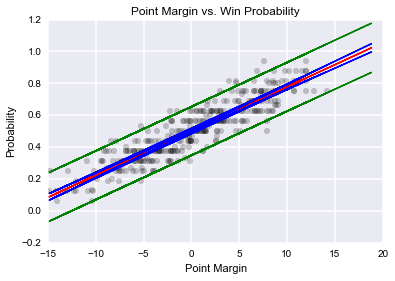
\includegraphics[max size={\textwidth}{\textheight}]{NFL-Go-For-It!_files/NFL-Go-For-It!_19_0.png}
    \par
    \end{center}
    
            \end{InvisibleVerbatim}
            
        
    
Creating a two matrices of the total points scored and total points let
go with the season as the column and the team as the row, and then
ranking them to get the offensive and defensive ranks.
After researching and deciding on our implementation method , we needed
to try and figure out a way to rank the teams 1 to 32 on offense and
defense (1 = best to 32 = worst). In order to rank teams first we
calculated the average number of points scored and given up per game per
season. The best offensive team for a particular season would be the
team that scored the most points per game. The best defensive team for a
particular season would be the team that gave up the fewest number of
points per game. Then, we plotted the number of points scored and given
up for the 32 teams per season. One could see that because our time
frame is rather long (11 years), the teams average number of points
scored and given up fluctuated greatly from season to season. For
example, the San Francisco 49ers went from one of the worst defenses in
the league in 2007 to one of the best in 2012.

Because fluctuations were so dramatic for the teams, we chose to rank
the teams 1 to 32 per season. So, the number one ranked offensive team
for example could change from the Patriots in 2002 to the Packers in
2003. After, we made this correction our plots of ranking and years look
much better for both offense and defense.The following is a plot of total points scored per season per team. Each
color represents a different team.

    

        % If the first block is an image, minipage the image.  Else
        % request a certain amount of space for the input text.
        \needspace{4\baselineskip}
        
        

            % Add document contents.
            
                \begin{InvisibleVerbatim}
                \vspace{-0.5\baselineskip}
    \begin{center}
    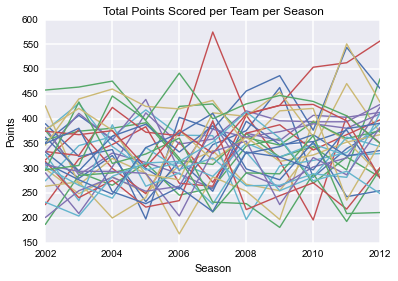
\includegraphics[max size={\textwidth}{\textheight}]{NFL-Go-For-It!_files/NFL-Go-For-It!_24_0.png}
    \par
    \end{center}
    
            \end{InvisibleVerbatim}
            
        
    
The following is a plot of total points let go per season per team. Each
color represents a different team.

    

        % If the first block is an image, minipage the image.  Else
        % request a certain amount of space for the input text.
        \needspace{4\baselineskip}
        
        

            % Add document contents.
            
                \begin{InvisibleVerbatim}
                \vspace{-0.5\baselineskip}
    \begin{center}
    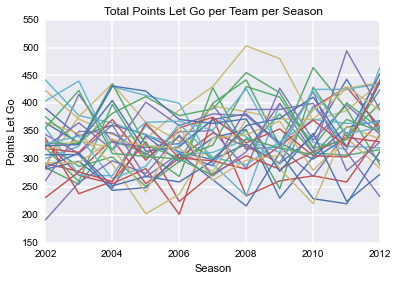
\includegraphics[max size={\textwidth}{\textheight}]{NFL-Go-For-It!_files/NFL-Go-For-It!_26_0.png}
    \par
    \end{center}
    
            \end{InvisibleVerbatim}
            
        
    
The graphs below show the top four and bottom two teams are many times
outliers in particular seasons. Many times the difference between these
outlying teams expected points is greater than the difference for the
teams in the middle. Because of this we created dummy variables, one for
those teams ranked 31 and 32, and one for those teams ranked 5 -- 30
(for both offense and defense). The dummy variable between 5 and 30 are
linearly related so we multiply this linear factor by the 5 -- 30 dummy.
However, teams 31 and 32 are close enough that we simply create a 0-1
dummy variable. Because of these dummies, our models are estimated in
comparison to offenses and defenses ranked 1-4.The following is a plot of total points scored per season per offensive
rank. Each color represents a different rank.

    

        % If the first block is an image, minipage the image.  Else
        % request a certain amount of space for the input text.
        \needspace{4\baselineskip}
        
        

            % Add document contents.
            
                \begin{InvisibleVerbatim}
                \vspace{-0.5\baselineskip}
    \begin{center}
    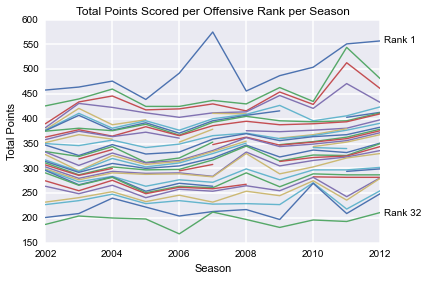
\includegraphics[max size={\textwidth}{\textheight}]{NFL-Go-For-It!_files/NFL-Go-For-It!_29_0.png}
    \par
    \end{center}
    
            \end{InvisibleVerbatim}
            
        
    
The following is a plot of total points scored per season per defensive
rank. Each color represents a different rank.

    

        % If the first block is an image, minipage the image.  Else
        % request a certain amount of space for the input text.
        \needspace{4\baselineskip}
        
        

            % Add document contents.
            
                \begin{InvisibleVerbatim}
                \vspace{-0.5\baselineskip}
    \begin{center}
    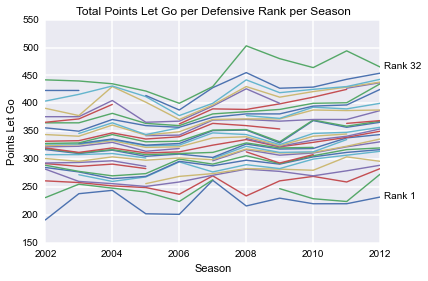
\includegraphics[max size={\textwidth}{\textheight}]{NFL-Go-For-It!_files/NFL-Go-For-It!_31_0.png}
    \par
    \end{center}
    
            \end{InvisibleVerbatim}
            
        
    
Here we bring in the team rankings into the main data frame.
Here we create dummy variables and factor variables concerning the
ranking of teams. This will help us run a logistic regression using team
ranking as covariates.


The following gives drive by drive information. This information is
useful in helping us know the expected number of points the offensive
team will score given they started the first play of the drive on a
specific yard line.
The following code quantifies the consequences of certain events
occurring. We create a vector of the number of points scored at the end
of a teams drive. We assume that touchdown plays automatically get seven
points, which means we assume the team gets the extra point given they
score a touchdown. Then we run a multinomial logistic regression to
determine the likelihood of these events based on certain factors, such
as team rank and field position. With both pieces of information we
determine the expected number points of a team given they convert a
first down, their ranking and their field position.

    

        % If the first block is an image, minipage the image.  Else
        % request a certain amount of space for the input text.
        \needspace{4\baselineskip}
        
        

            % Add document contents.
            
                \begin{InvisibleVerbatim}
                \vspace{-0.5\baselineskip}
\begin{alltt}Optimization terminated successfully.
         Current function value: 0.872453
         Iterations 12
\end{alltt}

            \end{InvisibleVerbatim}
            
                \makebox[0.1\linewidth]{\smaller\hfill\tt\color{nbframe-out-prompt}Out\hspace{4pt}{[}20{]}:\hspace{4pt}}\\*
                \vspace{-2.55\baselineskip}\begin{InvisibleVerbatim}
                \vspace{-0.5\baselineskip}
\begin{alltt}<class 'statsmodels.iolib.summary.Summary'>
"""
                          MNLogit Regression Results
======================================================================
========
Dep. Variable:                  score   No. Observations:
65105
Model:                        MNLogit   Df Residuals:
65081
Method:                           MLE   Df Model:
20
Date:                Wed, 30 Apr 2014   Pseudo R-squ.:
0.05169
Time:                        08:34:43   Log-Likelihood:
-56801.
converged:                       True   LL-Null:
-59897.
                                        LLR p-value:
0.000
======================================================================
==========
   score=DefTD       coef    std err          z      P>|z|      [95.0\%
Conf. Int.]
----------------------------------------------------------------------
------------
intercept         17.1021      1.159     14.759      0.000
14.831    19.373
ydline            -0.1892      0.012    -15.208      0.000
-0.214    -0.165
offrankMid         0.0065      0.010      0.620      0.535
-0.014     0.027
offrank31t32       0.0238      0.347      0.069      0.945
-0.656     0.704
defrankMid         0.0103      0.010      1.018      0.309
-0.010     0.030
defrank31t32       0.4581      0.395      1.161      0.246
-0.315     1.231
----------------------------------------------------------------------
------------
    score=FG       coef    std err          z      P>|z|      [95.0\%
Conf. Int.]
----------------------------------------------------------------------
----------
intercept       23.3837      1.125     20.785      0.000        21.179
25.589
ydline          -0.2381      0.012    -19.834      0.000        -0.262
-0.215
offrankMid      -0.0052      0.009     -0.565      0.572        -0.023
0.013
offrank31t32    -0.7413      0.308     -2.410      0.016        -1.344
-0.139
defrankMid       0.0217      0.009      2.428      0.015         0.004
0.039
defrank31t32     0.3214      0.357      0.901      0.368        -0.378
1.021
----------------------------------------------------------------------
----------
score=NoPoints       coef    std err          z      P>|z|      [95.0\%
Conf. Int.]
----------------------------------------------------------------------
------------
intercept         22.7030      1.124     20.200      0.000
20.500    24.906
ydline            -0.2050      0.012    -17.097      0.000
-0.228    -0.181
offrankMid         0.0080      0.009      0.870      0.384
-0.010     0.026
offrank31t32      -0.2494      0.303     -0.823      0.411
-0.844     0.345
defrankMid         0.0104      0.009      1.174      0.241
-0.007     0.028
defrank31t32       0.0488      0.354      0.138      0.890
-0.644     0.742
----------------------------------------------------------------------
------------
    score=TD       coef    std err          z      P>|z|      [95.0\%
Conf. Int.]
----------------------------------------------------------------------
----------
intercept       23.6977      1.125     21.070      0.000        21.493
25.902
ydline          -0.2343      0.012    -19.524      0.000        -0.258
-0.211
offrankMid      -0.0209      0.009     -2.270      0.023        -0.039
-0.003
offrank31t32    -1.3770      0.307     -4.487      0.000        -1.979
-0.775
defrankMid       0.0302      0.009      3.393      0.001         0.013
0.048
defrank31t32     0.7186      0.355      2.023      0.043         0.023
1.415
======================================================================
==========
"""\end{alltt}

            \end{InvisibleVerbatim}
            
        
    
The following is code concerning the decision to punt. Here, we find all
punt plays and using logistic regression we determine the probability of
events happening given that the team making the decision punted the ball
at a certain yard line. The other team receiveing the punt can then
score an offensive touchdown or field goal, get no points or give up a
defensive touchdown or safety.

    

        % If the first block is an image, minipage the image.  Else
        % request a certain amount of space for the input text.
        \needspace{4\baselineskip}
        
        

            % Add document contents.
            
                \begin{InvisibleVerbatim}
                \vspace{-0.5\baselineskip}
\begin{alltt}Optimization terminated successfully.
         Current function value: 0.881161
         Iterations 9
\end{alltt}

            \end{InvisibleVerbatim}
            
                \makebox[0.1\linewidth]{\smaller\hfill\tt\color{nbframe-out-prompt}Out\hspace{4pt}{[}21{]}:\hspace{4pt}}\\*
                \vspace{-2.55\baselineskip}\begin{InvisibleVerbatim}
                \vspace{-0.5\baselineskip}
\begin{alltt}<class 'statsmodels.iolib.summary.Summary'>
"""
                          MNLogit Regression Results
======================================================================
========
Dep. Variable:                  score   No. Observations:
26271
Model:                        MNLogit   Df Residuals:
26247
Method:                           MLE   Df Model:
20
Date:                Wed, 30 Apr 2014   Pseudo R-squ.:
0.03018
Time:                        08:34:46   Log-Likelihood:
-23149.
converged:                       True   LL-Null:
-23869.
                                        LLR p-value:
2.247e-293
======================================================================
===============
      score=DefTD       coef    std err          z      P>|z|
[95.0\% Conf. Int.]
----------------------------------------------------------------------
---------------
intercept            -2.5052      0.567     -4.415      0.000
-3.617    -1.393
removelast\_ydline     0.0502      0.009      5.741      0.000
0.033     0.067
offrankMid            0.0073      0.014      0.520      0.603
-0.020     0.035
offrank31t32         -0.1668      0.431     -0.387      0.699
-1.011     0.678
defrankMid            0.0189      0.013      1.431      0.153
-0.007     0.045
defrank31t32          0.2559      0.592      0.432      0.666
-0.905     1.417
----------------------------------------------------------------------
---------------
         score=FG       coef    std err          z      P>|z|
[95.0\% Conf. Int.]
----------------------------------------------------------------------
---------------
intercept            -2.0875      0.461     -4.532      0.000
-2.990    -1.185
removelast\_ydline     0.0874      0.007     11.719      0.000
0.073     0.102
offrankMid           -0.0018      0.012     -0.154      0.878
-0.024     0.021
offrank31t32         -0.9428      0.348     -2.712      0.007
-1.624    -0.262
defrankMid            0.0284      0.011      2.621      0.009
0.007     0.050
defrank31t32          0.6024      0.488      1.235      0.217
-0.354     1.558
----------------------------------------------------------------------
---------------
   score=NoPoints       coef    std err          z      P>|z|
[95.0\% Conf. Int.]
----------------------------------------------------------------------
---------------
intercept             1.3069      0.451      2.897      0.004
0.423     2.191
removelast\_ydline     0.0607      0.007      8.239      0.000
0.046     0.075
offrankMid            0.0132      0.011      1.160      0.246
-0.009     0.036
offrank31t32         -0.3978      0.338     -1.176      0.240
-1.061     0.265
defrankMid            0.0149      0.011      1.395      0.163
-0.006     0.036
defrank31t32          0.2583      0.482      0.536      0.592
-0.687     1.204
----------------------------------------------------------------------
---------------
         score=TD       coef    std err          z      P>|z|
[95.0\% Conf. Int.]
----------------------------------------------------------------------
---------------
intercept            -1.1274      0.457     -2.469      0.014
-2.022    -0.233
removelast\_ydline     0.0802      0.007     10.814      0.000
0.066     0.095
offrankMid           -0.0164      0.011     -1.428      0.153
-0.039     0.006
offrank31t32         -1.4860      0.346     -4.295      0.000
-2.164    -0.808
defrankMid            0.0381      0.011      3.529      0.000
0.017     0.059
defrank31t32          1.1201      0.485      2.311      0.021
0.170     2.070
======================================================================
===============
"""\end{alltt}

            \end{InvisibleVerbatim}
            
        
    
The following code is used to pull out fourth down plays from the data.
This is important since we'll use plays from these downs to find the
expected number of points given field goal attempt, punt attempt, or go
for it attempt.
Pulling out field goal attempt data and running a logistic regression to
determine the likelihood of converting depending on the yardline the
field goal is attempted from.

    

        % If the first block is an image, minipage the image.  Else
        % request a certain amount of space for the input text.
        \needspace{4\baselineskip}
        
        

            % Add document contents.
            
                \begin{InvisibleVerbatim}
                \vspace{-0.5\baselineskip}
\begin{alltt}Optimization terminated successfully.
         Current function value: 0.410096
         Iterations 7
\end{alltt}

            \end{InvisibleVerbatim}
            
                \makebox[0.1\linewidth]{\smaller\hfill\tt\color{nbframe-out-prompt}Out\hspace{4pt}{[}23{]}:\hspace{4pt}}\\*
                \vspace{-2.55\baselineskip}\begin{InvisibleVerbatim}
                \vspace{-0.5\baselineskip}
\begin{alltt}<class 'statsmodels.iolib.summary.Summary'>
"""
                           Logit Regression Results
======================================================================
========
Dep. Variable:              converted   No. Observations:
9650
Model:                          Logit   Df Residuals:
9648
Method:                           MLE   Df Model:
1
Date:                Wed, 30 Apr 2014   Pseudo R-squ.:
0.1206
Time:                        08:34:46   Log-Likelihood:
-3957.4
converged:                       True   LL-Null:
-4500.1
                                        LLR p-value:
5.246e-238
======================================================================
========
                 coef    std err          z      P>|z|      [95.0\%
Conf. Int.]
----------------------------------------------------------------------
--------
intercept      3.6030      0.083     43.532      0.000         3.441
3.765
ydline        -0.0981      0.003    -29.699      0.000        -0.105
-0.092
======================================================================
========
"""\end{alltt}

            \end{InvisibleVerbatim}
            
        
    

After evaluating and changing team ranks, a valid estimation of the
probabilities of conversion for field goals as well as fourth down
conversions must be performed. For each of these probabilities the
outcome is binary, either the kick or fourth down attempt was converted
or not. Therefore, we must implement a model that is used for a binary
response. The types of models that are most commonly performed in these
cases are logistic regression models or probit regression models. In our
particular case we will use the logistic regression model because our
model may not be normal, which is an assumption of the probit
regression. The assumptions of the logistic regression model are that
the response is binary, and the explanatory variables are independent.
Obviously, the response is binary, and we found no reason that in either
equation our explanatory variables were mutually related. Therefore, we
ran our models and computed 95 percent confidence intervals for given
situations.

From the graph below, it is obvious that the probability of a conversion
attempt is very close to 1 when it is a short kick (a kick with 0 yards
to your goal line, or a 17 yard field goal). This is not surprising at
all, because extra point attempts are from 20 yards away and kickers
make about 98 percent of extra point attempts. However, as one gets
further and further away it may surprise some people that the percentage
decrease for very long field goal attempts isn't more drastic. When you
have 50 yards to go (a 67-yard field goal) our model predicts about a 20
percent conversion rate. This obviously is too high; no one has ever
converted a field goal of longer than 63 yards. There are three major
reasons why these probabilities are clearly inflated. Firstly, only the
kickers with huge legs like Sebastian Janikowski kick field goals
greater than 60 yards. Secondly, they usually kick these field goals in
nice weather, possibly in Denver, where the altitude might give a kicker
5 or so yards of added range. And lastly, 67 yard field goals are not in
our data set. The logistic regression model does not accurately predict
response values when the explanatory variables are outside of the range
in the dataset. For these reasons, deep field goal probability
calculations are too high. From about the 40 yard line and in, however,
our results are more than believable. But, field goal success rate also
depends on your kicker and on the weather. These results average over
all kickers and different weather. If you are kicking in snow, or have a
terrible or great kicker, the coach should adjust the expected value of
kicking a field goal accordingly.The following graph has probabilities of converting field goals on the
y-axis and the yardline the field goal is attempted from. In the midterm
presentation the shading on the following graph was purely aesthetic.
After creating vectors of the standard errors the following graph now
contains the actual confidence interval.

    

        % If the first block is an image, minipage the image.  Else
        % request a certain amount of space for the input text.
        \needspace{4\baselineskip}
        
        

            % Add document contents.
            
                \begin{InvisibleVerbatim}
                \vspace{-0.5\baselineskip}
    \begin{center}
    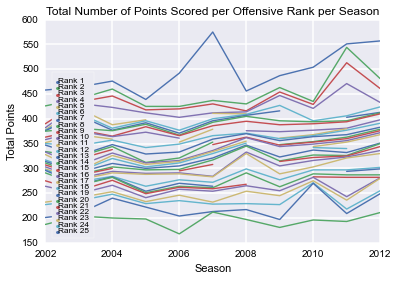
\includegraphics[max size={\textwidth}{\textheight}]{NFL-Go-For-It!_files/NFL-Go-For-It!_51_0.png}
    \par
    \end{center}
    
            \end{InvisibleVerbatim}
            
        
    
In the following cell we create binary columns in the fourth down play
data set to indicate what decision was made on the fourth down.
First off, we must explain fourth downs in our data set. Because all
fourth quarter plays were extracted from our data set, and the
prevailing conventional wisdom is to not attempt fourth downs unless it
is a late game situation, there weren't enough fourth down plays to make
accurate predictions. Therefore, we accounted for this by calculating
the probability of third down conversion. This seems odd, but in today's
NFL, the third down is of a similar mind set to fourth down if you went
for it. Teams aggressively try and convert the first because they nearly
always punt if they do not convert. There are however, some third down
situations that are not similar to fourth down situations. For instance,
many times on third and long, teams will run the ball and concede
punting just to not throw an interception or create more room for their
punter. In these situations, if it was fourth down they would obviously
be going more aggressively for the first. Because of this, all third
down plays of greater than 10 yards which were runs were taken out of
the model. We felt these observations would bias our results.

After using these particular plays to model fourth down plays, we know
that the probability of a fourth down conversion should change depending
on the strength of the offense and opposing teams' defense, the number
of yards to go for a first down, and the field position. From our model,
you can see that as the yards to go increases the probability decreases.
Also, the better the offense is in comparison to the defense increases
the probability of conversion. And the yard line we turned into a
categorical variable. This categorical variable indicates whether the
fourth down conversion is from the other teams' 0 -- 10, 10 -- 30, or
30-50 yard line, or your own 0-10, 10-30, or 30-50 yard line. You can
see from these probabilities that the conversion rate from the other
teams' 0-10 is lowest (it is the one left out of the equation) because
all the numbers are positive. Then, as one might expect the conversion
rate if you have greater than 90 yards to go is lower in relation to the
other yard lines as well because teams are nervous about safety
possibilities and other factors.The following pulls out the rankings of teams and yards to go to convert
on the fourth down. We also perform a logistic regression to determine
the likelihood of converting given the rankings and yards to go. Third
down plays are used in the logistic regression since using the fourth
down plays gives a bias in the estimate.

    

        % If the first block is an image, minipage the image.  Else
        % request a certain amount of space for the input text.
        \needspace{4\baselineskip}
        
        

            % Add document contents.
            
                \begin{InvisibleVerbatim}
                \vspace{-0.5\baselineskip}
\begin{alltt}Optimization terminated successfully.
         Current function value: 0.639043
         Iterations 5
\end{alltt}

            \end{InvisibleVerbatim}
            
                \makebox[0.1\linewidth]{\smaller\hfill\tt\color{nbframe-out-prompt}Out\hspace{4pt}{[}27{]}:\hspace{4pt}}\\*
                \vspace{-2.55\baselineskip}\begin{InvisibleVerbatim}
                \vspace{-0.5\baselineskip}
\begin{alltt}<class 'statsmodels.iolib.summary.Summary'>
"""
                           Logit Regression Results
======================================================================
========
Dep. Variable:              converted   No. Observations:
72787
Model:                          Logit   Df Residuals:
72776
Method:                           MLE   Df Model:
10
Date:                Wed, 30 Apr 2014   Pseudo R-squ.:
0.06244
Time:                        08:34:49   Log-Likelihood:
-46514.
converged:                       True   LL-Null:
-49612.
                                        LLR p-value:
0.000
======================================================================
==========
                   coef    std err          z      P>|z|      [95.0\%
Conf. Int.]
----------------------------------------------------------------------
----------
intercept        0.3322      0.035      9.441      0.000         0.263
0.401
togo            -0.1417      0.002    -68.676      0.000        -0.146
-0.138
ydline10t30      0.2740      0.035      7.912      0.000         0.206
0.342
ydline30t50      0.4415      0.033     13.261      0.000         0.376
0.507
ydline50t70      0.4682      0.032     14.554      0.000         0.405
0.531
ydline70t90      0.4394      0.033     13.149      0.000         0.374
0.505
ydline90t100     0.3284      0.063      5.242      0.000         0.206
0.451
offrankMid      -0.0136      0.001    -15.401      0.000        -0.015
-0.012
offrank31t32    -0.4547      0.036    -12.807      0.000        -0.524
-0.385
defrankMid       0.0062      0.001      7.073      0.000         0.005
0.008
defrank31t32     0.2090      0.035      5.922      0.000         0.140
0.278
======================================================================
==========
"""\end{alltt}

            \end{InvisibleVerbatim}
            
        
    

convert\_prob is a three dimensional matrix that gives the probability
of the offensive team converting a first down given how many yards to go
for the first down, the offensive rank of the offense and the defensive
rank of the defense.

The following shows the probability of conversion of first down per
offensive and defensive rankings with 1 yard to go.

    

        % If the first block is an image, minipage the image.  Else
        % request a certain amount of space for the input text.
        \needspace{4\baselineskip}
        
        

            % Add document contents.
            
                \begin{InvisibleVerbatim}
                \vspace{-0.5\baselineskip}
    \begin{center}
    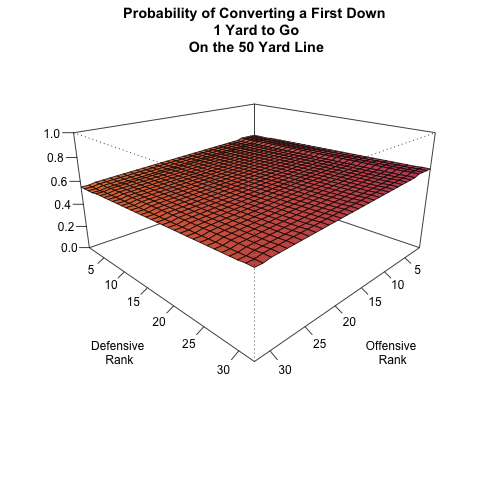
\includegraphics[max size={\textwidth}{\textheight}]{NFL-Go-For-It!_files/NFL-Go-For-It!_62_0.png}
    \par
    \end{center}
    
            \end{InvisibleVerbatim}
            
        
    
The following shows the probability of conversion of first down per
offensive and defensive rankings with 3 yard to go.

    

        % If the first block is an image, minipage the image.  Else
        % request a certain amount of space for the input text.
        \needspace{4\baselineskip}
        
        

            % Add document contents.
            
                \begin{InvisibleVerbatim}
                \vspace{-0.5\baselineskip}
    \begin{center}
    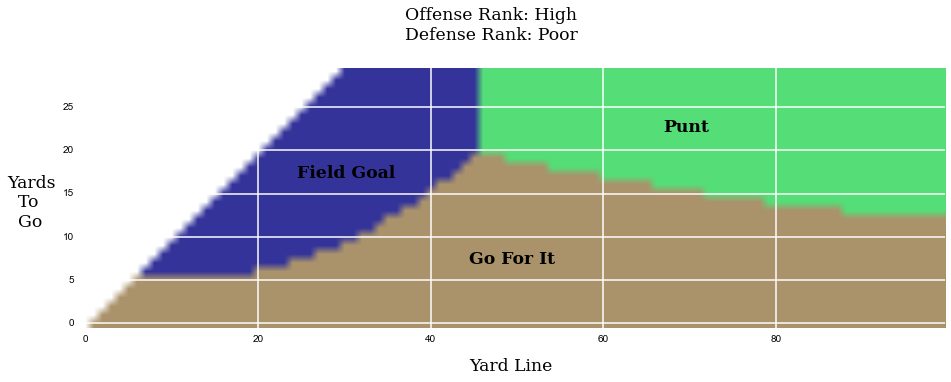
\includegraphics[max size={\textwidth}{\textheight}]{NFL-Go-For-It!_files/NFL-Go-For-It!_64_0.png}
    \par
    \end{center}
    
            \end{InvisibleVerbatim}
            
        
    
The following shows the probability of conversion of first down per
offensive and defensive rankings with 6 yard to go.

    

        % If the first block is an image, minipage the image.  Else
        % request a certain amount of space for the input text.
        \needspace{4\baselineskip}
        
        

            % Add document contents.
            
                \begin{InvisibleVerbatim}
                \vspace{-0.5\baselineskip}
    \begin{center}
    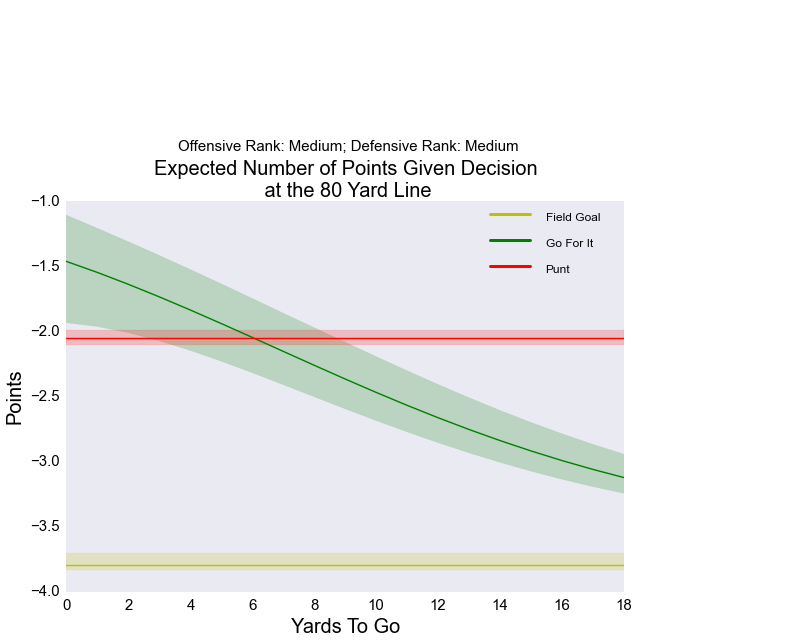
\includegraphics[max size={\textwidth}{\textheight}]{NFL-Go-For-It!_files/NFL-Go-For-It!_66_0.png}
    \par
    \end{center}
    
            \end{InvisibleVerbatim}
            
        
    
The following shows the probability of conversion of first down per
offensive and defensive rankings with 9 yard to go.

    

        % If the first block is an image, minipage the image.  Else
        % request a certain amount of space for the input text.
        \needspace{4\baselineskip}
        
        

            % Add document contents.
            
                \begin{InvisibleVerbatim}
                \vspace{-0.5\baselineskip}
    \begin{center}
    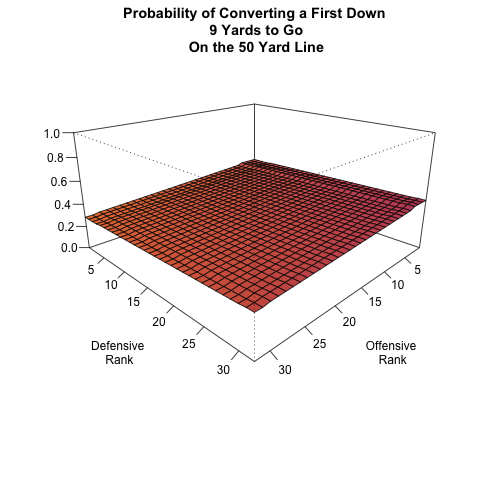
\includegraphics[max size={\textwidth}{\textheight}]{NFL-Go-For-It!_files/NFL-Go-For-It!_68_0.png}
    \par
    \end{center}
    
            \end{InvisibleVerbatim}
            
        
    


    

        % If the first block is an image, minipage the image.  Else
        % request a certain amount of space for the input text.
        \needspace{4\baselineskip}
        
        

            % Add document contents.
            
                \begin{InvisibleVerbatim}
                \vspace{-0.5\baselineskip}
    \begin{center}
    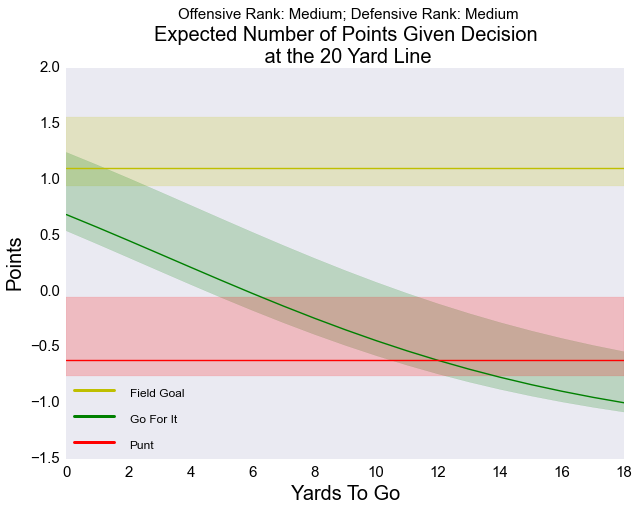
\includegraphics[max size={\textwidth}{\textheight}]{NFL-Go-For-It!_files/NFL-Go-For-It!_69_0.png}
    \par
    \end{center}
    
            \end{InvisibleVerbatim}
            
        
    
The following graph gives one particular example, of the effect of the
number of yards to go on the probability conversion. This graph assumes
that the offense and opposing teams defense are both near average (15th
and 15th ranked), and the team making the decision is on the 50 yard
line. You can clearly see that the probability of conversion is about .7
with one or fewer yards to go, and steadily goes down to about .1 with
20 yards to go. These numbers are pretty consistent with the numbers
published in a few papers about league average (fourth and less than 1
is about .68) (according to one paper I read -- need to find it!).

    

        % If the first block is an image, minipage the image.  Else
        % request a certain amount of space for the input text.
        \needspace{4\baselineskip}
        
        

            % Add document contents.
            
                \begin{InvisibleVerbatim}
                \vspace{-0.5\baselineskip}
    \begin{center}
    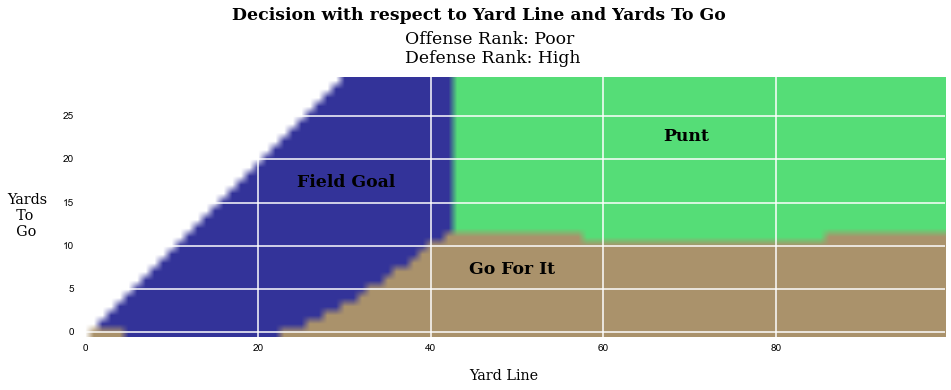
\includegraphics[max size={\textwidth}{\textheight}]{NFL-Go-For-It!_files/NFL-Go-For-It!_71_0.png}
    \par
    \end{center}
    
            \end{InvisibleVerbatim}
            
        
    
If the offensive team's rank is high (5th) and the defensive rank is low
(25th) one can see that the probability increases slightly when
comparing across yards to go from the previous plot. Instead of the
graph steadily decreasing from about .68 to .1 (0 to 20 yards away), the
probabilities range from .72 to .14.

    

        % If the first block is an image, minipage the image.  Else
        % request a certain amount of space for the input text.
        \needspace{4\baselineskip}
        
        

            % Add document contents.
            
                \begin{InvisibleVerbatim}
                \vspace{-0.5\baselineskip}
    \begin{center}
    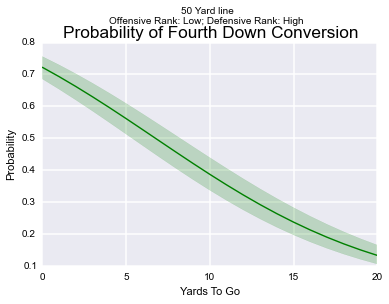
\includegraphics[max size={\textwidth}{\textheight}]{NFL-Go-For-It!_files/NFL-Go-For-It!_73_0.png}
    \par
    \end{center}
    
            \end{InvisibleVerbatim}
            
        
    

The expected number of points is calculated by multiplying the possible
outcomes of a drive by the point values given those outcomes. In each
drive there are five possible outcomes: a touchdown or field goal scored
by the offense, a safety or touchdown scored by the defense, and no
points. These numbers are multiplied by the points of each outcome: 7,
3, -2, -7, and 0 respectively. For the model, we assume every touchdown
is 7 points (not 6 or 8) which is true the vast majority of the time. In
order to estimate the probabilities of these outcomes we decided to use
a multinomial logistic regression model. A multinomial model is used for
a categorical response variable (here five categories) when the
explanatory variables are independent. Here, the explanatory variables
for our model are the offensive rank and the defensive rank of the two
respective teams as well as the starting field position. The assumption
of independence seems reasonable.

If you notice, the calculations can get complicated if for instance the
team who decides to punt gets a defensive touchdown on the other teams
next drive. Or, if the opposing team to the one making the decision
scores a safety because they get the ball back on offense after this
play. These two situations were accounted for and implemented by simply
multiplying the probability of the safety or defensive touchdown by the
expected values of the next drive. By accounting for these possibilities
we ensure that the observations are consistent.\\

From the multinomial and logistic calculations, we can calculate the
expected point values given each decision. Then a confidence interval is
computed for each of the three scenarios by taking each of the lower
bounds and upper bounds of the combined intervals and adding them
together. Because of the complexities in this calculation the estimated
line is not in the middle of the confidence interval. Also, this
interval is technically greater than 95 percent because we are combining
other 95 percent confidence intervals.The following functions will be used to determine the choice to be made
given yard line, yards to go, and both offensive and defensive rankings
of the team making the decision as well as the other team.







The next plots illustrate how the yard-line affects the optimal
decision, with given offensive and defensive ranks of both the team
making the decision and the opposing team (all ranks around 15). In the
first plot the optimal decision is to kick a field goal regardless of
the number of yards to go. However, with less than one yard to go the
confidence intervals overlap which means it may be optimal to go for the
first down. The coach should make the final decision if the intervals
overlap. With 50 yards to go, and the same rankings, the optimal
decision changes in a pretty major way. Now, the graph indicates that a
team should go for the first down on fourth and less than 6, between 6
and 12 yards either punt or go for it, and past 12 yards punt. From a
team's own 20 yard line (80 yards to the goal line), a team's optimal
decision is to go for it on fourth and less than 3, either punt or go
for it between 3 and 9 yards to go, and punt the ball if there are more
than 9 yards to go for a first.The following is the plot of the decision that should be made from the
50 yard line, where the offensive team has an mediocre ranking and the
defensive team is ranked mediocre.


    

        % If the first block is an image, minipage the image.  Else
        % request a certain amount of space for the input text.
        \needspace{4\baselineskip}
        
        

            % Add document contents.
            
                \begin{InvisibleVerbatim}
                \vspace{-0.5\baselineskip}
    \begin{center}
    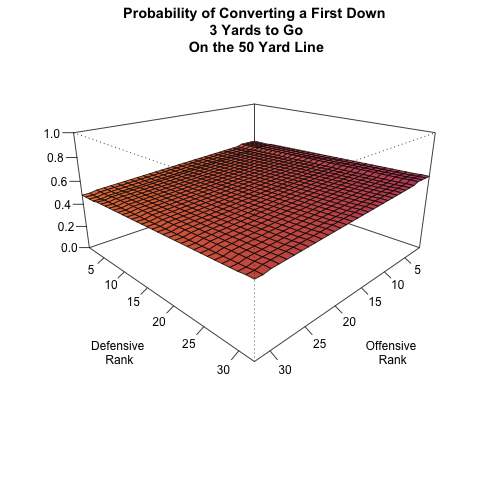
\includegraphics[max size={\textwidth}{\textheight}]{NFL-Go-For-It!_files/NFL-Go-For-It!_88_0.png}
    \par
    \end{center}
    
            \end{InvisibleVerbatim}
            
        
    
The following is the plot of the decision that should be made from the
80 yard line, where the offensive team has an mediocre ranking and the
defensive team is ranked mediocre.


    

        % If the first block is an image, minipage the image.  Else
        % request a certain amount of space for the input text.
        \needspace{4\baselineskip}
        
        

            % Add document contents.
            
                \begin{InvisibleVerbatim}
                \vspace{-0.5\baselineskip}
    \begin{center}
    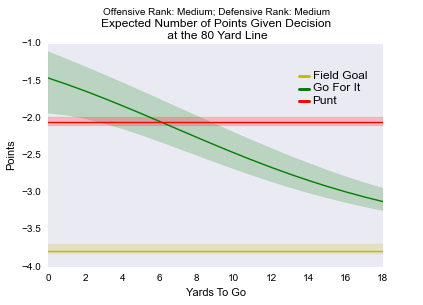
\includegraphics[max size={\textwidth}{\textheight}]{NFL-Go-For-It!_files/NFL-Go-For-It!_91_0.png}
    \par
    \end{center}
    
            \end{InvisibleVerbatim}
            
        
    
The following is the plot of the decision that should be made from the
20 yard line, where the offensive team has a mediocre ranking and the
defensive team is ranked mediocre.


    

        % If the first block is an image, minipage the image.  Else
        % request a certain amount of space for the input text.
        \needspace{4\baselineskip}
        
        

            % Add document contents.
            
                \begin{InvisibleVerbatim}
                \vspace{-0.5\baselineskip}
    \begin{center}
    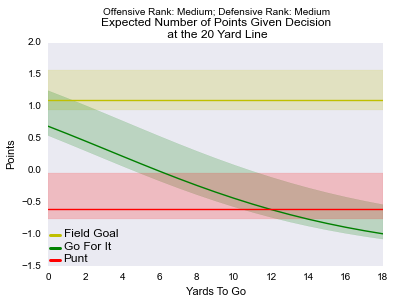
\includegraphics[max size={\textwidth}{\textheight}]{NFL-Go-For-It!_files/NFL-Go-For-It!_94_0.png}
    \par
    \end{center}
    
            \end{InvisibleVerbatim}
            
        
    







    

        % If the first block is an image, minipage the image.  Else
        % request a certain amount of space for the input text.
        \needspace{4\baselineskip}
        
        

            % Add document contents.
            
                \begin{InvisibleVerbatim}
                \vspace{-0.5\baselineskip}
    \begin{center}
    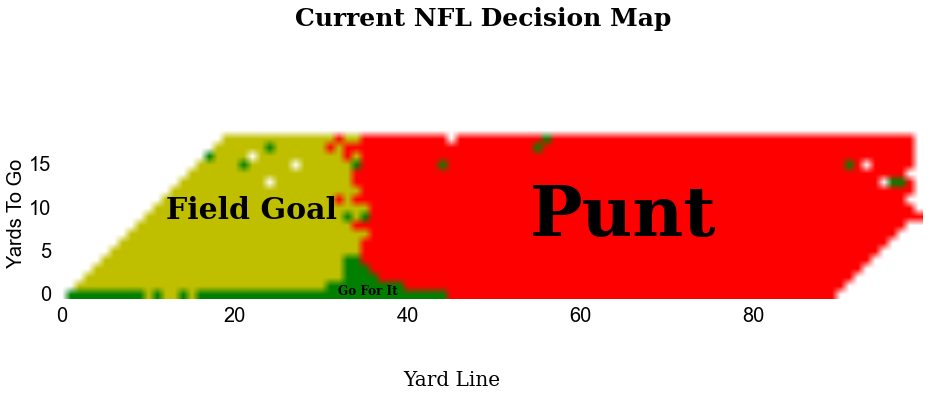
\includegraphics[max size={\textwidth}{\textheight}]{NFL-Go-For-It!_files/NFL-Go-For-It!_100_0.png}
    \par
    \end{center}
    
            \end{InvisibleVerbatim}
            
        
    
This progression is common to all offensive and defensive ranks. The 3
charts below paint the picture for the optimal decision for every
position on the field and any fourth down situation less than 20 yards
to go for certain rankings of the offensive and defensive units of both
teams. If the team making the decision has a high ranking offense and
defense, and the opposing team has a low ranking offense and defense,
the optimal decision in many circumstances is to go for it. Our
calculations project that it is optimal to attempt the first down
anywhere on the field which is fourth and less than 2. The optimal
decision map also indicates that you should go for it from about fourth
and 15 from the 50, as well as fourth and 7 from your own 3. These
numbers are obviously very surprising, but they are partially high
because of the unusually large difference between the teams' rankings.The following gives the decision to be made given high ranking of the
offensive team and poor ranking of the defensive team.


    

        % If the first block is an image, minipage the image.  Else
        % request a certain amount of space for the input text.
        \needspace{4\baselineskip}
        
        

            % Add document contents.
            
                \begin{InvisibleVerbatim}
                \vspace{-0.5\baselineskip}
    \begin{center}
    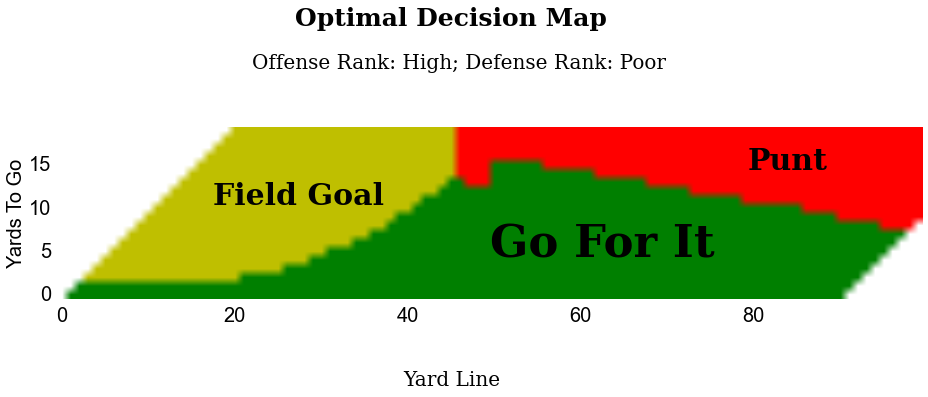
\includegraphics[max size={\textwidth}{\textheight}]{NFL-Go-For-It!_files/NFL-Go-For-It!_104_0.png}
    \par
    \end{center}
    
            \end{InvisibleVerbatim}
            
        
    
If the teams are ranked evenly for both offense and defense then our map
become more conservative. Now, the map indicates that a team should
attempt the first down conversion from fourth and 8 with 50 yards to go
and fourth and 4 with 96 yards to go to the goal line.The following gives the decision to be made given mediocre ranking of
the offensive team and mediocre ranking of the defensive team.


    

        % If the first block is an image, minipage the image.  Else
        % request a certain amount of space for the input text.
        \needspace{4\baselineskip}
        
        

            % Add document contents.
            
                \begin{InvisibleVerbatim}
                \vspace{-0.5\baselineskip}
    \begin{center}
    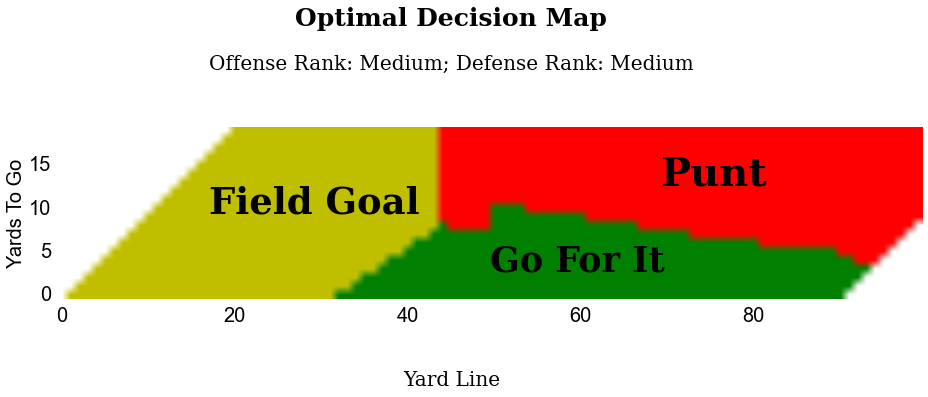
\includegraphics[max size={\textwidth}{\textheight}]{NFL-Go-For-It!_files/NFL-Go-For-It!_108_0.png}
    \par
    \end{center}
    
            \end{InvisibleVerbatim}
            
        
    
The optimal decision map becomes even more conservative when the team
making the decision is weak on both offense and defense, and the
opposing team is strong offensively and defensively. Now, the decision
map's optimal values are to go for the first down on fourth and four
from the 50, and go for it on fourth and one with 91 yards to go to the
goal line.The following gives the decision to be made given poor ranking of the
offensive team and high ranking of the defensive team.


    

        % If the first block is an image, minipage the image.  Else
        % request a certain amount of space for the input text.
        \needspace{4\baselineskip}
        
        

            % Add document contents.
            
                \begin{InvisibleVerbatim}
                \vspace{-0.5\baselineskip}
    \begin{center}
    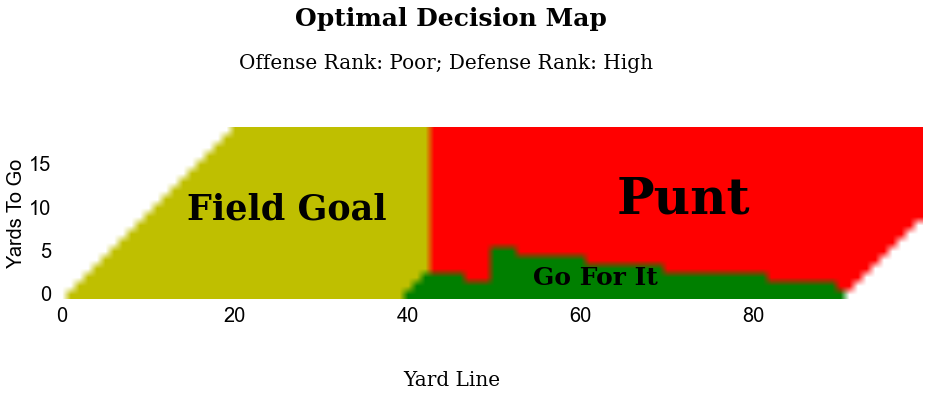
\includegraphics[max size={\textwidth}{\textheight}]{NFL-Go-For-It!_files/NFL-Go-For-It!_112_0.png}
    \par
    \end{center}
    
            \end{InvisibleVerbatim}
            
        
    
Obviously, the ranking of both teams' offense and defense have an
enormous impact on the optimal decision. For a high ranking offense, a
coach should go for it much more often given other rankings remain
constant. The dramatic changes in these plots purely due to teams'
offensive and defensive ranks are interesting, but how does the overall
trend compare to current NFL fourth down decision making may be a better
question? The plot below shows the decisions coaches and upper
management have made over these 11 seasons. When comparing the maps,
there are stark differences from our previous three optimal decision
maps. The first major difference is that teams rarely go for it. In fact
anywhere past the 45 yard line the decision most often made in every
scenario (combination of yard line and yards to go) is to punt. One
other noticeable feature is that our earlier plots had kickers going for
a field goal attempt from much larger distances. Once again, this value
is heavily inflated because of the higher than should be conversion rate
of deep attempts.

Our analysis should not convince you that the results we obtained are
perfect. The data used in our analysis is observational, and there is no
way to prove causality. Therefore, coaches' deep level of knowledge of
the game should still play a major role in determining the fourth down
decision. But, their football expertise along with an understanding of
the estimated expected values could help guide their decision under
uncertainty. The stark difference between our logical model and the
current NFL's usual decision is obvious. We still would not recommend
going for a first down on fourth and seven from your own 3 yard line.
However, our process makes intuitive and mathematical sense. And the
optimal decision is most likely somewhere in the middle. Obviously,
giving up possession of the ball by punting has a much greater negative
effect than teams currently realize.

The model could be improved, and the assumptions fortified with the help
of other statistician gurus. But, this is a good start in showing that
something is off. The way current NFL coaches and upper management
evaluate fourth down decisions is seriously flawed. In the next decade,
statistics will probably play a more integral role in fourth down
decision making because the first few teams that makes sense of the data
will have a distinct advantage.
        

        \renewcommand{\indexname}{Index}
        \printindex

    % End of document
    \end{document}


